%%%%%%%%%%%%%%%%%%%%%%%%%%%%%%%%%%%%%%%%%
% Sullivan Business Report
% LaTeX Template
% Version 1.0 (May 5, 2022)
%
% This template originates from:
% https://www.LaTeXTemplates.com
%
% Author:
% Vel (vel@latextemplates.com)
%
% License:
% CC BY-NC-SA 4.0 (https://creativecommons.org/licenses/by-nc-sa/4.0/)
%
%%%%%%%%%%%%%%%%%%%%%%%%%%%%%%%%%%%%%%%%%


%----------------------------------------------------------------------------------------
%	CLASS, PACKAGES AND OTHER DOCUMENT CONFIGURATIONS
%----------------------------------------------------------------------------------------

\documentclass[
    a4paper, % Paper size, use either a4paper or letterpaper
	12pt, % Default font size, the template is designed to look good at 12pt so it's best not to change this
	%unnumberedsections, % Uncomment for no section numbering
    ]{CSSullivanBusinessReport}
    
    \addbibresource{sample.bib} % BibLaTeX bibliography file

%----------------------------------------------------------------------------------------
%	REPORT INFORMATION
%----------------------------------------------------------------------------------------

\reporttitle{CPE 233 Hardware Assignment 4} % The report title is to appear on the title page and page headers, do not create manual new lines here as this will carry over to page headers

\reportsubtitle{Arithmetic Logic Unit and Immediate Generator Design and Verification} % Report subtitle, include new lines if needed

\reportauthors{Report by:\\\smallskip Ethan Vosburg (evosburg@calpoly.edu)} % Report authors/group/department, include new lines if needed

\reportdate{\today} % Report date, include new lines for additional information if needed

\rightheadercontent{
\includegraphics[width=3cm]{creodocs_logo.pdf}} % The content in the right header, you may want to add your own company logo or use your company/department name or leave this command empty for no right header content

%----------------------------------------------------------------------------------------

\begin{document}

%----------------------------------------------------------------------------------------
%	TITLE PAGE
%----------------------------------------------------------------------------------------

\thispagestyle{empty} % Suppress headers and footers on this page

\begin{fullwidth} % Use the whole page width
	\vspace*{-0.075\textheight} % Pull logo into the top margin
	
	\hfill
\includegraphics[width=5cm]{creodocs_logo.pdf} % Company logo

	\vspace{0.15\textheight} % Vertical whitespace

	\parbox{0.9\fulltextwidth}{\fontsize{50pt}{52pt}\selectfont\raggedright\textbf{\reporttitle}\par} % Report title, intentionally at less than full width for nice wrapping. Adjust the width of the \parbox and the font size as needed for your title to look good.
	
	\vspace{0.03\textheight} % Vertical whitespace
	
	{\LARGE\textit{\textbf{\reportsubtitle}}\par} % Subtitle
	
	\vfill % Vertical whitespace
	
	{\Large\reportauthors\par} % Report authors, group or department
	
	\vfill\vfill\vfill % Vertical whitespace
	
	{\large\reportdate\par} % Report date
\end{fullwidth}

\newpage

%----------------------------------------------------------------------------------------
%	DISCLAIMER/COPYRIGHT PAGE
%----------------------------------------------------------------------------------------

% \thispagestyle{empty} % Suppress headers and footers on this page

% \begin{twothirdswidth} % Content in this environment to be at two-thirds of the whole page width
% 	\footnotesize % Reduce font size
	
% 	\subsection*{Disclaimer}

% 	Lorem ipsum dolor sit amet, consectetur adipiscing elit. Praesent porttitor arcu luctus, imperdiet urna iaculis, mattis eros. Pellentesque iaculis odio vel nisl ullamcorper, nec faucibus ipsum molestie. Sed dictum nisl non aliquet porttitor. Etiam vulputate arcu dignissim, finibus sem et, viverra nisl. Aenean luctus congue massa, ut laoreet metus ornare in. Nunc fermentum nisi imperdiet lectus tincidunt vestibulum at ac elit.
	
% 	\subsection*{Copyright}
	
% 	\textcopyright~[Year] [Company] 
	
% 	Copyright notice text\ldots In hac habitasse platea dictumst. Curabitur mattis elit sit amet justo luctus vestibulum. In hac habitasse platea dictumst. Pellentesque lobortis justo enim, a condimentum massa tempor eu. Ut quis nulla a quam pretium eleifend nec eu nisl. Nam cursus porttitor eros, sed luctus ligula convallis quis.
	
% 	\subsection*{Contact}
	
% 	Address Line 1\\
% 	Address Line 2\\
% 	Address Line 3
	
% 	Business Number 123456
	
% 	Contact: name@company.com
	
% 	\vfill % Push the following down to the bottom of the page
	
% 	\subsubsection*{Changelog}
	
% 	\scriptsize % Reduce font size further
	
% 	\begin{tabular}{@{} L{0.05\linewidth} L{0.15\linewidth} L{0.6\linewidth} @{}} % Column widths specified here, change as needed for your content
% 		\toprule
% 		v1.0 & 20XX-02-05 & Lorem ipsum dolor sit amet, consectetur adipiscing elit. Praesent porttitor arcu luctus, imperdiet urna iaculis, mattis eros.\\
% 		v1.1 & 20XX-02-27 & Pellentesque iaculis odio vel nisl ullamcorper, nec faucibus ipsum molestie.\\
% 		v1.2 & 20XX-03-15 & Sed dictum nisl non aliquet porttitor.\\
% 		\bottomrule
% 	\end{tabular}
% \end{twothirdswidth}

% \newpage

%----------------------------------------------------------------------------------------
%	TABLE OF CONTENTS
%----------------------------------------------------------------------------------------
\bigskip
\begin{twothirdswidth} % Content in this environment to be at two-thirds of the whole page width
	\tableofcontents % Output the table of contents, automatically generated from the section commands used in the document
\end{twothirdswidth}

\newpage

%----------------------------------------------------------------------------------------
%	SECTIONS
%----------------------------------------------------------------------------------------
\begin{fullwidth} % Use the whole page width

\section{Project Description} % Top level section

In this project, an Arithmetic Logic Unit (ALU) and an Immediate Generator were designed and verified. The ALU is a combinational circuit that performs arithmetic and logic operations on two 32-bit inputs. The Immediate Generator is a combinational circuit that generates a 32-bit immediate value from a multi-bit immediate value. The ALU and Immediate Generator were designed using System Verilog and then verified using a testbench.

\section{Structural Design} % Second level section

\subsection{Arithmetic Logic Unit Elaborated Design} % Third level section

\begin{figure}[H]
    \centering
    \captionsetup{style=widetable}
    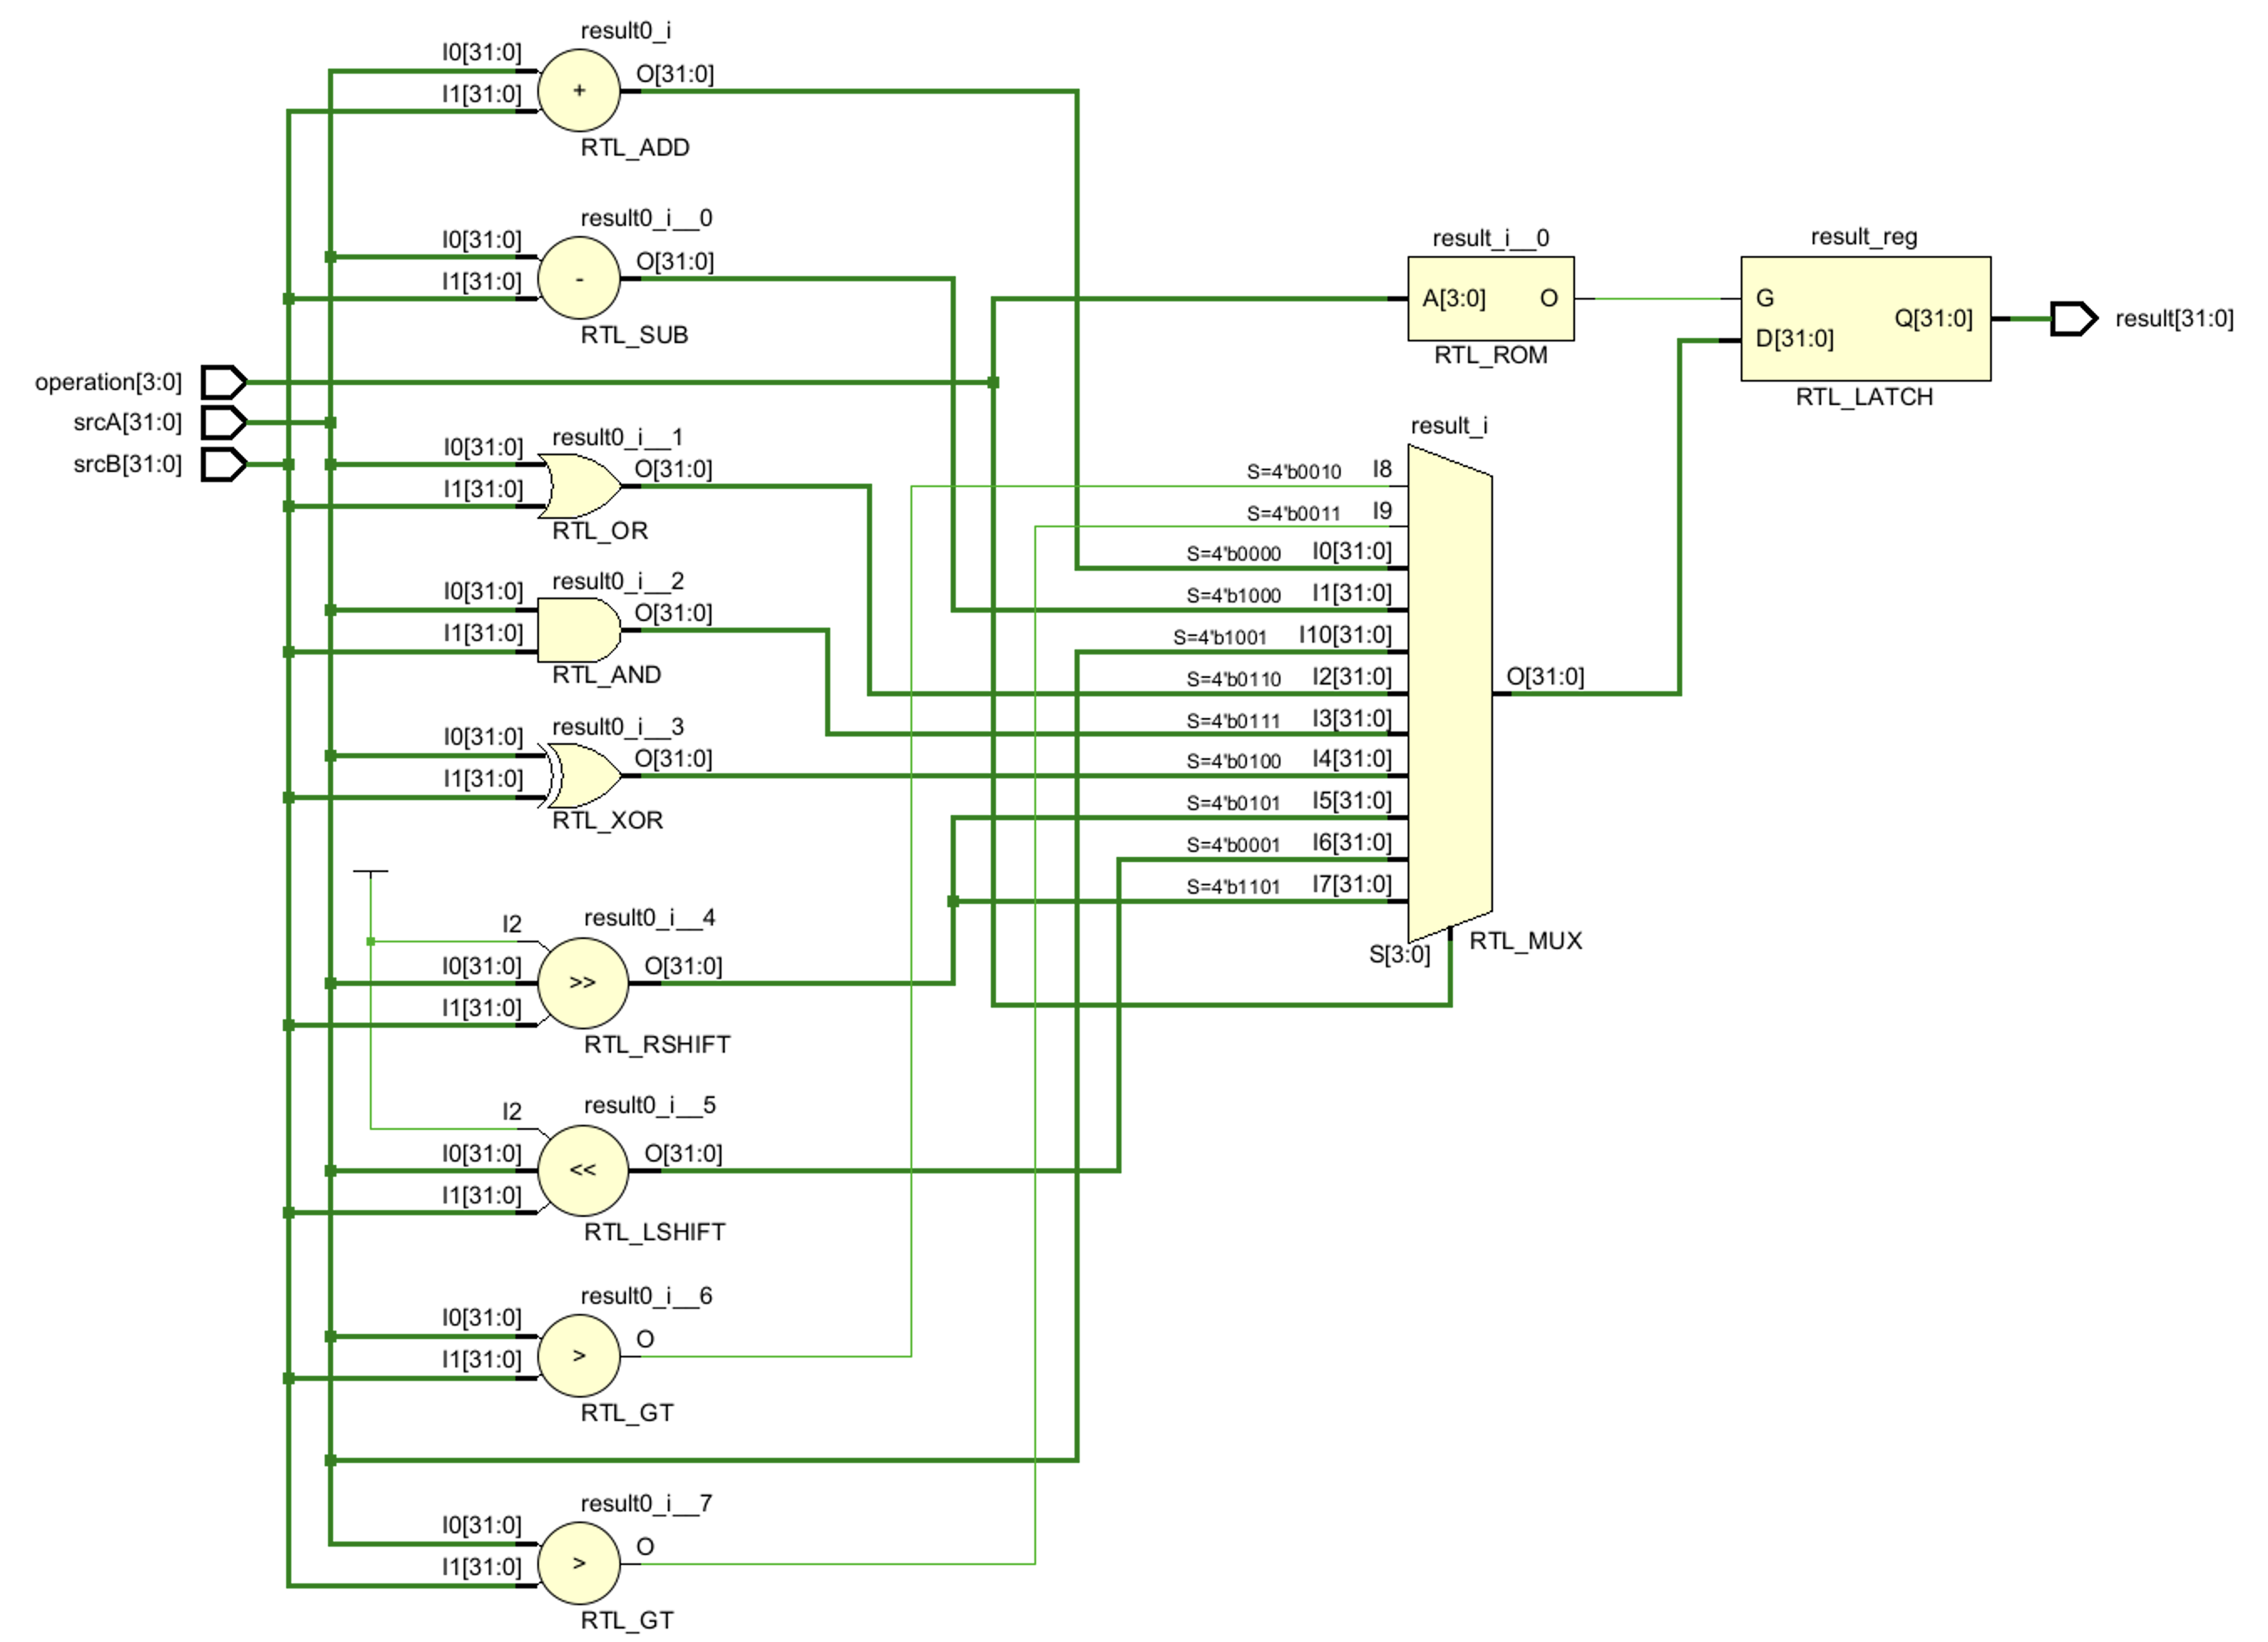
\includegraphics[width=.80\pdfpagewidth]{Figures/ALU-Elaborated-Design.png}
    \caption{Arithmetic Logic Unit Elaborated Design}
    \label{fig:ALUElaboratedDesign}
\end{figure}

\subsection{Immediate Generator Elaborated Design} % Third level section
\begin{figure}[H]
    \centering
    \captionsetup{style=widetable}
    \makebox[.80\pdfpagewidth]{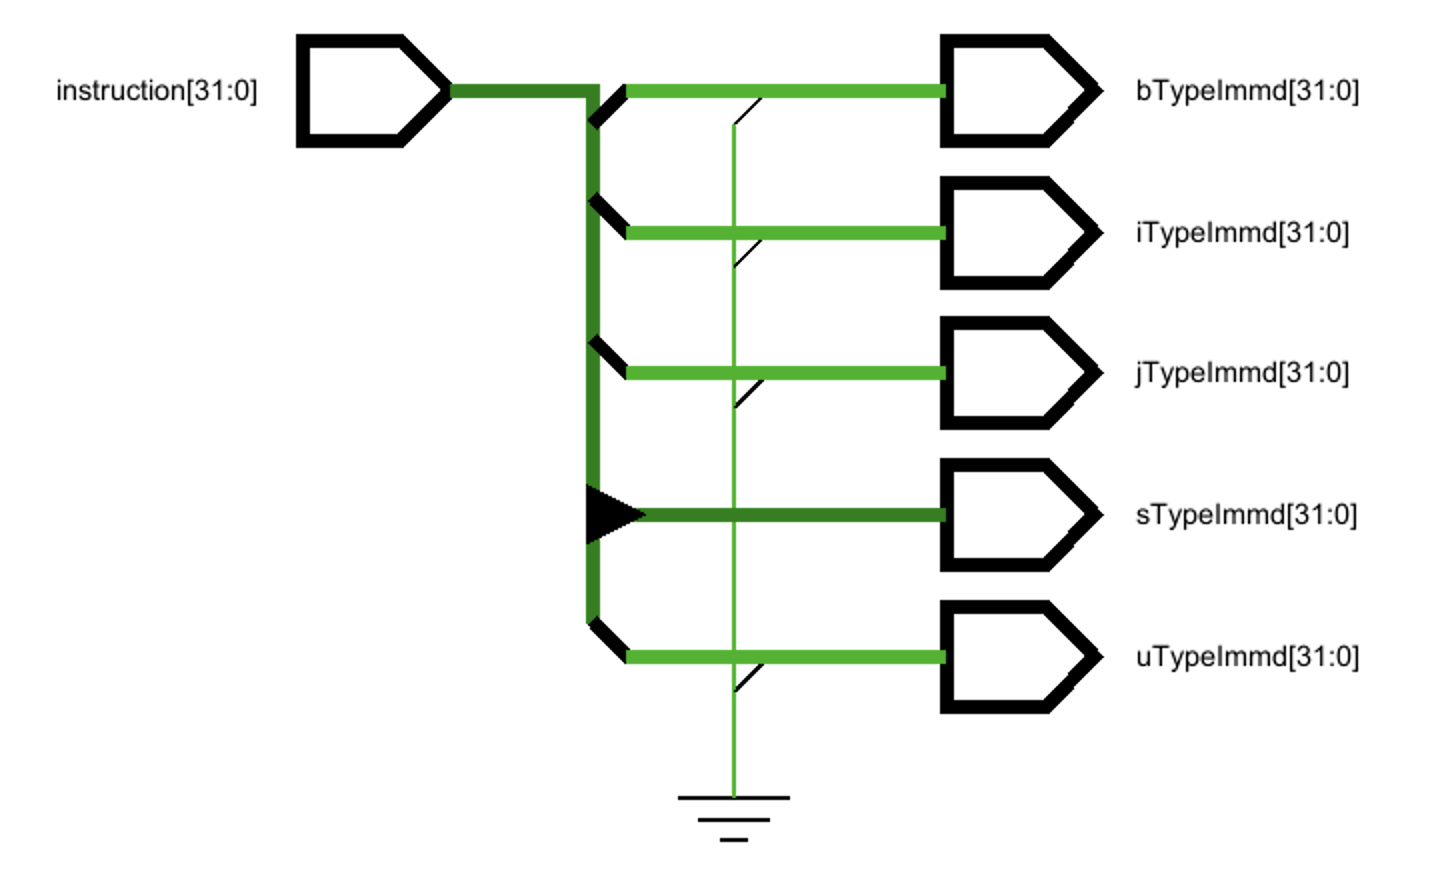
\includegraphics[width=.50\pdfpagewidth]{Figures/Immediate-Generator-Elaborated Design.png}}
    \caption{Immediate Generator Elaborated Design}
    \label{fig:ALUElaboratedDesign}
\end{figure}


\section{Synthesis Warnings} % Second level section

\subsection{Arithmetic Logic Unit Synthesis Warnings} % Third level section
\begin{figure}[H]
    \captionsetup{style=widetable}
    \makebox[.80\pdfpagewidth]{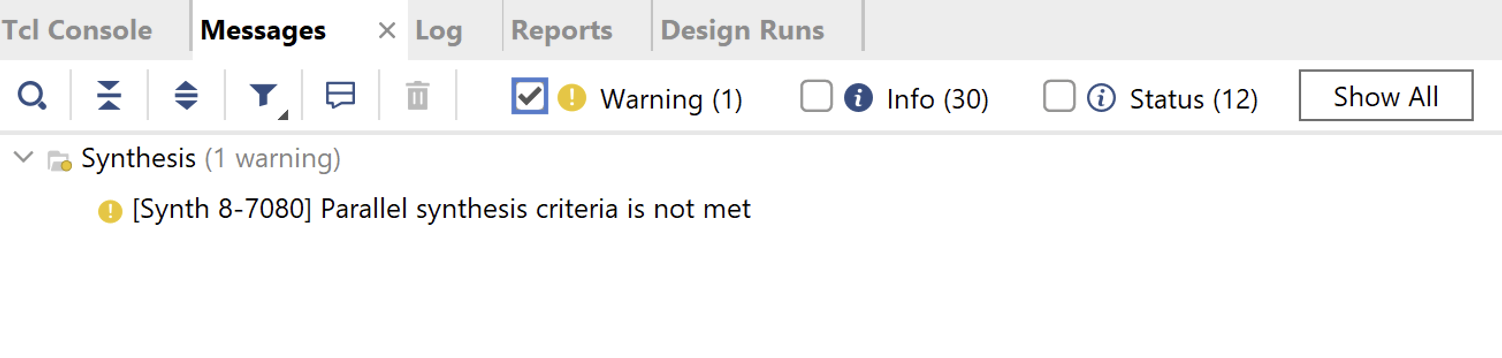
\includegraphics[width=.75\pdfpagewidth]{Figures/Zero Console Warnings.png}}
    \caption{Arithmetic Logic Unit Synthesis Warnings}
    \label{fig:ALUSynthesisWarnings}
\end{figure}

\subsection{Immediate Generator Synthesis Warnings} % Third level section
\begin{figure}[H]
    \captionsetup{style=widetable}
    \makebox[.80\pdfpagewidth]{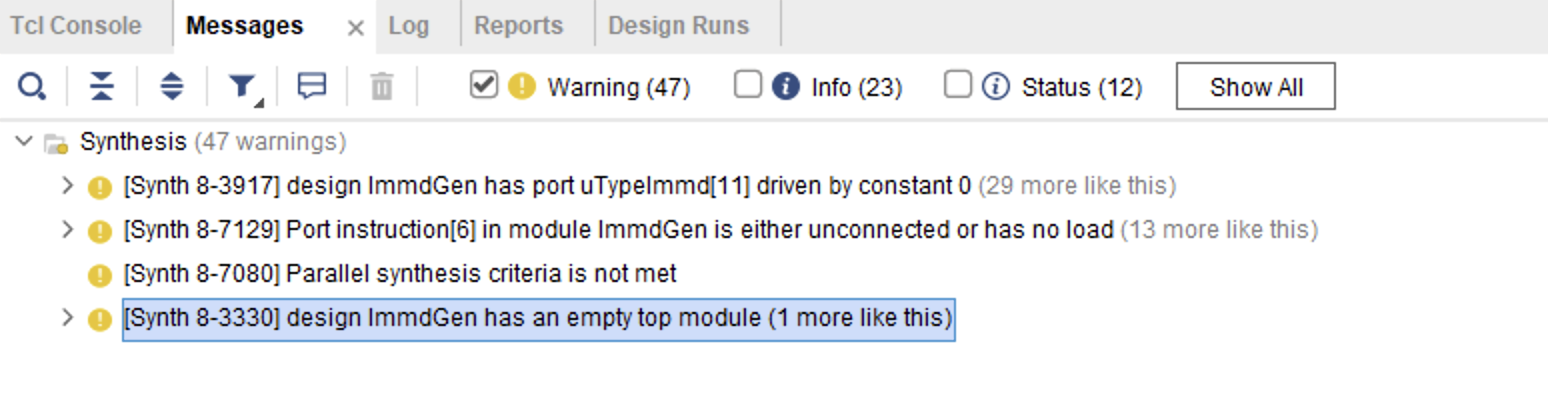
\includegraphics[width=.75\pdfpagewidth]{Figures/ImmdGen Console Warnings.png}}
    \caption{Immediate Generator Synthesis Warnings}
    \label{fig:ImmdGenSynthesisWarnings}
\end{figure}

The three warning messages that came up in figure \ref{fig:ImmdGenSynthesisWarnings} are not concerning. Warning \\\verb|Synth 8-3917| references a constant driving the output of the module. This is expected because we are padding the immediate values with zeros which are constants. Warning \verb|Synth 8-7129| is also not a concern as to maintain the same terminology as the RiscV specification for the immediate values, the first 7 bits of the input to the immediate generator are not used. Warning \verb|Synth 8-3330| is also not a concern since this module is simply parsing an immediate value and is not performing logic. Finally, warning \verb|Synth 7080| is not a concern as we are not performing parallel synthesis.  
\section{Verification} % Second level section

\subsection{Arithmetic Logic Unit Testbench Coverage} % Third level section

The testbench for the ALU was designed to test many of the edge cases of the ALU as well as make sure that every operation was tested in a way where all of the bits in and out were either 1 or 0 for at least one operation. The testbench was able to verify that the ALU worked properly and passed all of the test cases.

\subsection{Immediate Generator Testbench Coverage} % Third level section


\begin{enumerate}
    \item \textbf{U Type} For testing the U Type immediate, several test cases were made in RARS to test the maximum and minimum values of the immediate as well as make sure every bit could be a 1 or a 0.
    \item \textbf{I Type} For testing the I Type immediate, several test cases were made in RARS to test the maximum and minimum values of the immediate as well as make sure every bit could be a 1 or a 0.
    \item \textbf{S Type} For testing the S Type immediate, several test cases were made in RARS to test the maximum and minimum values of the immediate as well as make sure every bit could be a 1 or a 0.
    \item \textbf{S Type} For testing the S Type immediately, several values were tested as well as changing the sign extension of some values to make sure the sign extension was working properly.
    \item \textbf{B Type} For the B Type immediate, a similar approach was taken as with the S Type where the sign extension was tested as well as several values.
\end{enumerate}

\captionsetup{style=widetable}
\subsection{Arithmetic Logic Unit Testbench Code} % Third level section?

\lstinputlisting[language=Verilog, caption=System Verilod Testbench Code for Arithmetic Logic Unit]{/Users/ethanvosburg/Documents/git/CPE-233-Otter/HW4-ALU-ImmedGen/HW4-ALU-ImmedGen/HW4-ALU-ImmedGen.srcs/sim_1/new/ALU_TB.sv}

\newpage
\lstinputlisting[language=Verilog, caption=System Verilog Arithmetic Logic Unit Test Case File]{/Users/ethanvosburg/Documents/git/CPE-233-Otter/HW4-ALU-ImmedGen/HW4-ALU-ImmedGen/HW4-ALU-ImmedGen.srcs/sources_1/imports/HW4-ALU-ImmedGen/aluVerification.mem}

\newpage
\subsection {Immediate Generator Testbench Code} % Third level section
\lstinputlisting[language=Verilog, caption=System Verilog Immediate Generator Testbench]{/Users/ethanvosburg/Documents/git/CPE-233-Otter/HW4-ALU-ImmedGen/HW4-ALU-ImmedGen/HW4-ALU-ImmedGen.srcs/sim_1/new/ImmdGen_TB.sv}

\lstinputlisting[language=Verilog, caption=System Verilog Immediate Generator Testbench]{/Users/ethanvosburg/Documents/git/CPE-233-Otter/HW4-ALU-ImmedGen/HW4-ALU-ImmedGen/HW4-ALU-ImmedGen.srcs/sources_1/imports/HW4-ALU-ImmedGen/ImmdGenVerification.mem}


\newpage
\subsection{Arithmetic Logic Unit Testbench Output} % Third level section
Running this testbench produced the following output in the TCL code console:
\begin{table}[H]
    \centering
    % \captionsetup{justification=centering}
    \footnotesize
    \captionsetup{style=widetable}
    \caption{Flow Chart 1 Test Cases}
    \begin{tabular}{|c||l|c|c|c|}
    % \begin{tabular}{|c|c|}
    \hline
     ALU FUN &ALU\_SEL&A& B& Output\\\hline
    \hline
    ADD&0000&0xA50F96C3& 0x5AF0693C& 0xffffffff\\\hline
    &0000&0x84105F21& 0x7B105FDE& 0xff20beff\\\hline
    &0000&0xFFFFFFFF& 0x00000001& 0x00000000\\\hline
    \hline
    SUB&1000& 0x00000000& 0x00000001&0xffffffff\\\hline
    &1000& 0xAA806355& 0x550162AA& 0x557f00ab\\\hline
    &1000& 0x550162AA& 0xAA806355&0xaa80ff55\\\hline
    \hline
    AND&0111& 0xA55A00FF& 0x5A5AFFFF&0x005a00ff\\\hline
    &0111& 0xC3C3F966& 0xFF669F5A&0xc3429942\\\hline
    \hline
    OR&0110& 0x9A9AC300& 0x65A3CC0F&0xffbbcf0f\\\hline
    &0110& 0xC3C3F966& 0xFF669F5A&0xffe7ff7e\\\hline
    \hline
    XOR&0100& 0xAA5500FF& 0x5AA50FF0&0xf0f00f0f\\\hline
    &0100& 0xA5A56C6C& 0xFF00C6FF&0x5aa5aa93\\\hline
    \hline
    SRL&0101& 0x805A6CF3& 0x00000010&0x0000805a\\\hline
    &0101& 0x705A6CF3& 0x00000005&0x0382d367\\\hline
    &0101& 0x805A6CF3& 0x00000000&0x805a6cf3\\\hline
    &0101& 0x805A6CF3& 0x00000100&0x00000000\\\hline
    \hline
    SLL&0001& 0x805A6CF3& 0x00000010&0x6cf30000\\\hline
    &0001& 0x805A6CF3& 0x00000005&0x0b4d9e60\\\hline
    &0001& 0x805A6CF3& 0x00000100&0x00000000\\\hline
    \hline
    SRA&1101& 0x805A6CF3& 0x00000010&0x0000805a\\\hline
    &1101& 0x705A6CF3& 0x00000005&0x0382d367\\\hline
    &1101& 0x805A6CF3& 0x00000000&0x805a6cf3\\\hline
    &1101& 0x805A6CF3& 0x00000100&0x00000000\\\hline
    \hline
    SLT&0010& 0x7FFFFFFF& 0x80000000&0x00000000\\\hline
    &0010& 0x80000000& 0x00000001&0x00000001\\\hline
    &0010& 0x00000000& 0x00000000&0x00000000\\\hline
    &0010& 0x55555555& 0x55555555&0x00000000\\\hline
    \hline
    SLTU&0011& 0x7FFFFFFF& 0x80000000&0x00000001\\\hline
    &0011& 0x80000000& 0x00000001&0x00000000\\\hline
    &0011& 0x00000000& 0x00000000&0x00000000\\\hline
    &0011& 0x55AA55AA& 0x55AA55AA&0x00000000\\\hline
    \hline
    LUI COPY&1001& 0x01234567& 0x76543210&0x01234567\\\hline
    &1001& 0xFEDCBA98& 0x89ABCDEF&0xfedcba98\\\hline
    \end{tabular}
\end{table}

\newpage
\subsection{Immediate Generator Testbench Output} % Third level section
\lstinputlisting[language=Verilog, caption=Verilog Code for Arithmetic Logic Unit]{/Users/ethanvosburg/Documents/git/CPE-233-Otter/HW4-ALU-ImmedGen/ImmdGenTestCase.txt}

\newpage
\subsection{Simulation Results} % Third level section

Running this testbench produced the following simulation results:

\begin{figure}[H]
    \centering
    \captionsetup{style=widetable}
    \makebox[.80\pdfpagewidth]{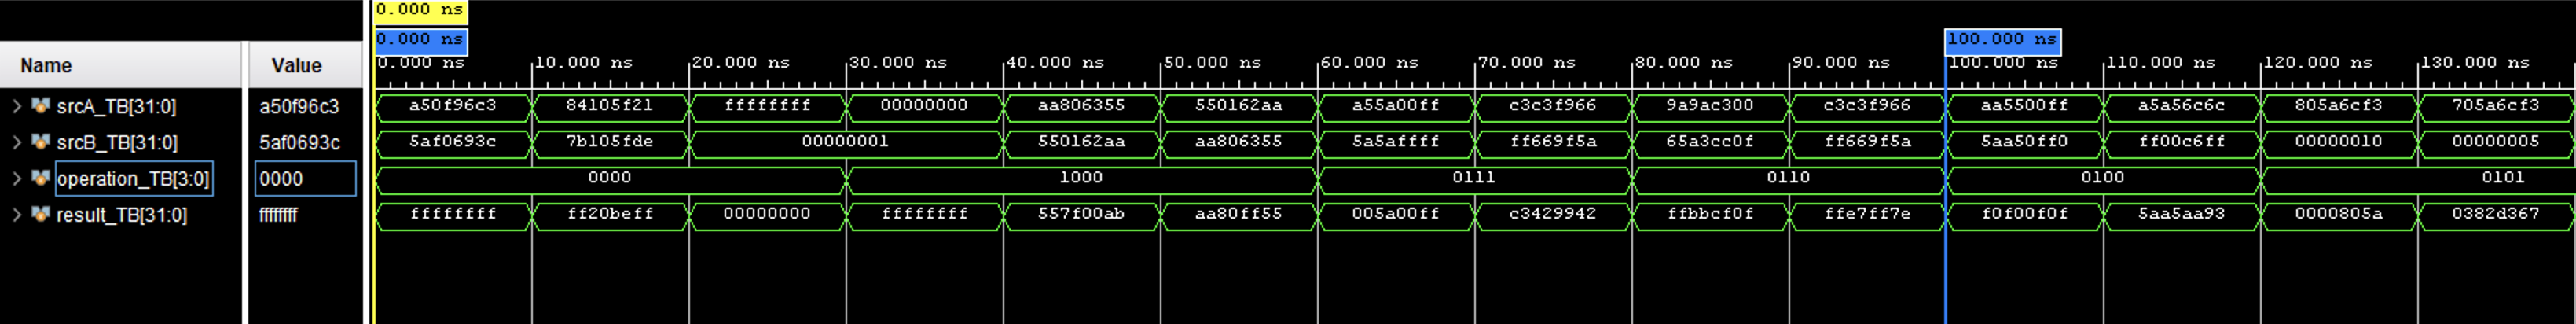
\includegraphics[width=.8\pdfpagewidth]{Figures/ALU-Simulation-0.png}}
    \caption{Arithmetic Logic Unit Simulation 0ns - 100ns}
    \label{fig:ALUSim0}
\end{figure}

\begin{figure}[H]
    \centering
    \captionsetup{style=widetable}
    \makebox[.80\pdfpagewidth]{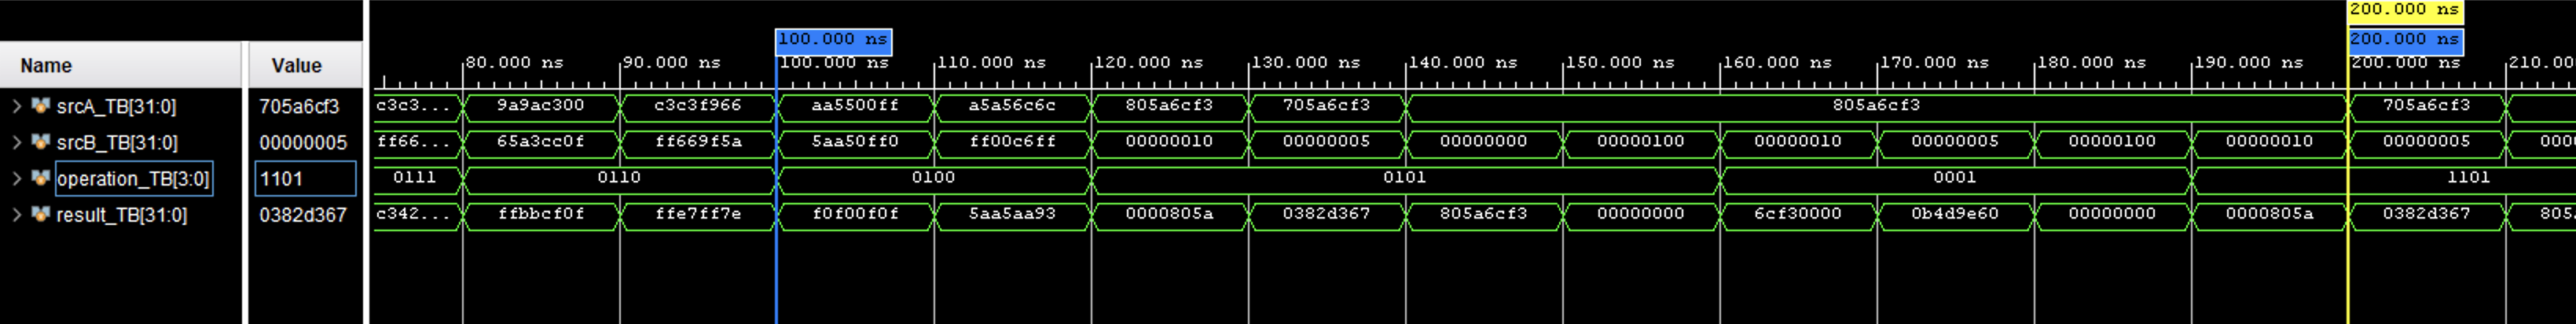
\includegraphics[width=.8\pdfpagewidth]{Figures/ALU-Simulation-1.png}}
    \caption{Arithmetic Logic Unit Simulation 100ns - 200ns}
    \label{fig:ALUSim1}
\end{figure}

\begin{figure}[H]
    \centering
    \captionsetup{style=widetable}
    \makebox[.80\pdfpagewidth]{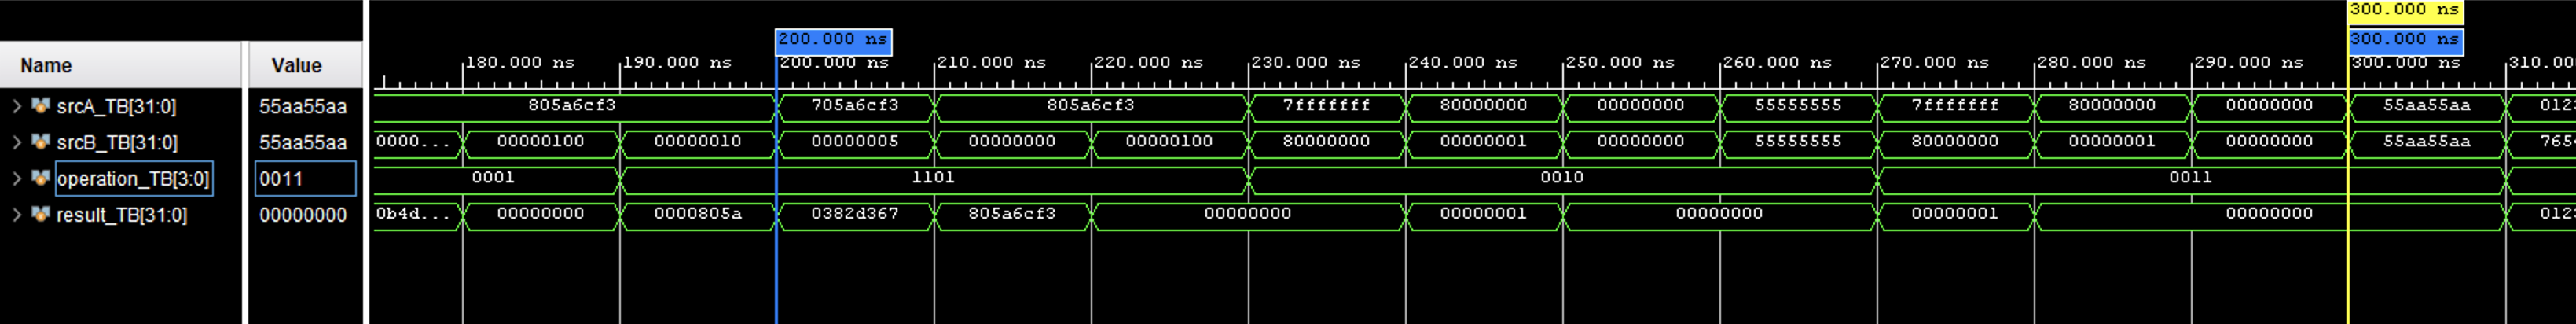
\includegraphics[width=.8\pdfpagewidth]{Figures/ALU-Simulation-2.png}}
    \caption{Arithmetic Logic Unit Simulation 200ns - 300ns}
    \label{fig:ALUSim2}
\end{figure}

\begin{figure}[H]
    \centering
    \captionsetup{style=widetable}
    \makebox[.80\pdfpagewidth]{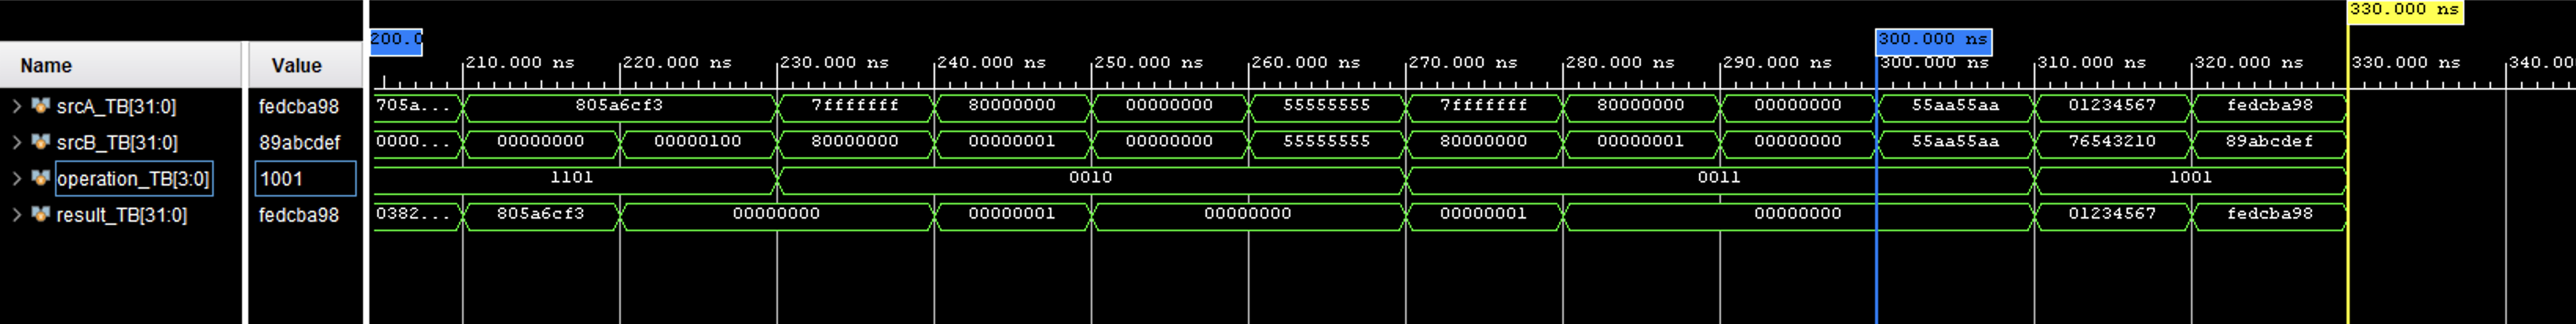
\includegraphics[width=.8\pdfpagewidth]{Figures/ALU-Simulation-3.png}}
    \caption{Aritmetic Logic Unit Simulation 300ns - 330ns}
    \label{fig:ALUSim3}
\end{figure}

\begin{figure}[H]
    \centering
    \captionsetup{style=widetable}
    \makebox[.80\pdfpagewidth]{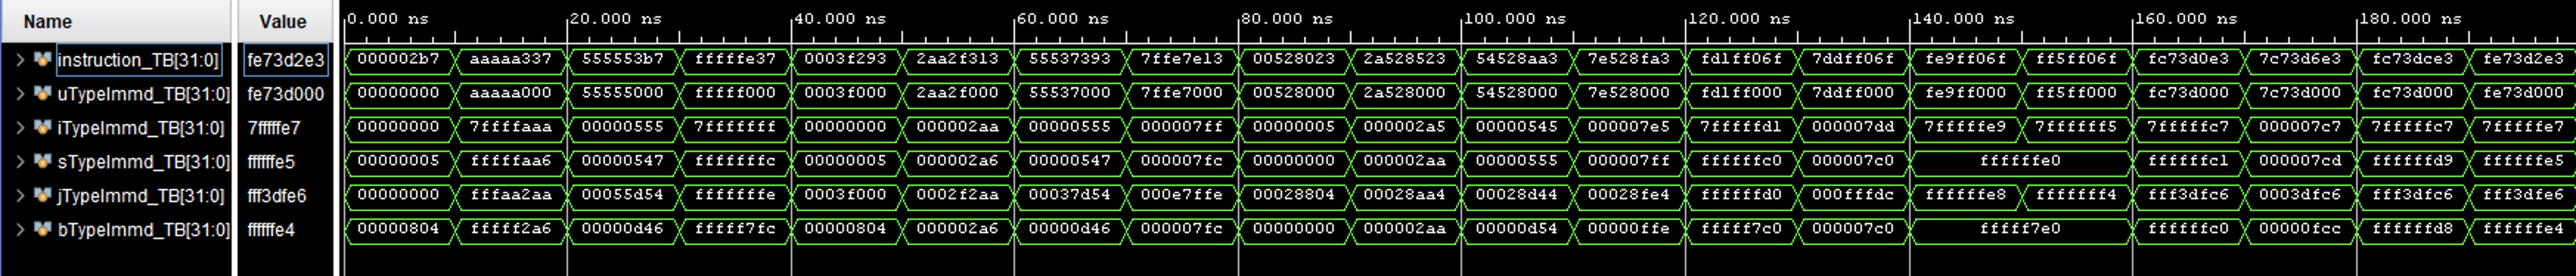
\includegraphics[width=.8\pdfpagewidth]{Figures/ImmdGen Simulation.png}}
    \caption{Immediate Generator Simulation 0ns - 200ns}
    \label{fig:ImmdGenSim0}
\end{figure}

\newpage
\section{Source Code}
\captionsetup{style=widetable}
\subsection{Arithmetic Logic Unit} % Third level section

\lstinputlisting[language=Verilog, caption=Verilog Code for Arithmetic Logic Unit]{/Users/ethanvosburg/Documents/git/CPE-233-Otter/HW4-ALU-ImmedGen/HW4-ALU-ImmedGen/HW4-ALU-ImmedGen.srcs/sources_1/new/ALU.sv}

\newpage
\subsection{Immediate Generator} % Third level section

\lstinputlisting[language=Verilog, caption=Verilog Code for Immediate Generator]{/Users/ethanvosburg/Documents/git/CPE-233-Otter/HW4-ALU-ImmedGen/HW4-ALU-ImmedGen/HW4-ALU-ImmedGen.srcs/sources_1/new/ImmdGen.sv}

\newpage



\section {Conclusion} % Second level section
\hypersetup{urlcolor=blue} 
The arithmetic logic unit is the heart of the Otter processor and performs all of the actions as described by the RiscV specification. The immediate generator is equally important and parses all of the immediate values that are frequently fed into the ALU. In this project, an ALU and immediate generator were created and tested. Through the verification process, both modules were tested and passed all test cases showing that there is reasonable confidence that the modules will work as expected in the Otter processor. 
All code for this assignment can be found \href{https://github.com/EthanV1920/CPE-233-Otter/tree/main}{here}.


\end{fullwidth}

\end{document}